\documentclass[12pt, a4paper, oneside]{ctexart}
\usepackage{amsmath, amsthm, amssymb, bm, color, graphicx, geometry, mathrsfs,extarrows, braket, booktabs, array, wrapfig}
\usepackage[colorlinks,linkcolor=red,anchorcolor=blue,citecolor=blue,urlcolor=blue,menucolor=black]{hyperref}
%%%% 设置中文字体 %%%%
\setCJKmainfont{方正新书宋_GBK.ttf}[BoldFont=方正小标宋_GBK, ItalicFont=方正楷体_GBK]
%%%% 设置英文字体 %%%%
\setmainfont{Times New Roman}
\setsansfont{Calibri}
\setmonofont{Consolas}

\linespread{1.4}
%\geometry{left=2.54cm,right=2.54cm,top=3.18cm,bottom=3.18cm}
\geometry{left=1.84cm,right=1.84cm,top=2.18cm,bottom=2.18cm}
\newcounter{problem}  % 问题序号计数器
\newenvironment{problem}[1][]{\stepcounter{problem}\par\noindent\textbf{题目\arabic{problem}. #1}}{\smallskip\par}
\newenvironment{solution}[1][]{\par\noindent\textbf{#1解答. }}{\smallskip\par}  % 可带一个参数表示题号\begin{solution}{题号}
\newenvironment{note}{\par\noindent\textbf{注记. }}{\smallskip\par}

%%%% 图片相对路径 %%%%
\graphicspath{{figure/}} % 当前目录下的figure文件夹, {../figure/}则是父目录的figure文件夹
\setlength{\abovecaptionskip}{-0.2cm}  % 缩紧图片标题与图片之间的距离
\setlength{\belowcaptionskip}{0pt} 

\usepackage{minted}
\renewcommand{\theFancyVerbLine}{
    \sffamily\textcolor[rgb]{0.5,0.5,0.5}{\scriptsize\arabic{FancyVerbLine}}} % 修改代码前序号大小
\newmintinline{cpp}{fontsize=\small, linenos, breaklines, frame=lines}  % 使用\cppinline{代码}
\newminted{cpp}{fontsize=\small, linenos, breaklines, frame=lines}  % 使用\begin{cppcode}代码\end{cppcode}
\newmintinline{python}{fontsize=\small, linenos, breaklines, frame=lines, python3}  % 使用\pythoninline{代码}
\newminted{python}{fontsize=\small, linenos, breaklines, frame=lines, python3}  % 使用\begin{pythoncode}代码\end{pythoncode}
\newmintedfile{python}{fontsize=\small, linenos, breaklines, frame=lines, python3}  % 使用\pythonfile{代码地址}


\everymath{\displaystyle} % 默认全部行间公式
\DeclareMathOperator*\uplim{\overline{lim}} % 定义上极限 \uplim_{}
\DeclareMathOperator*\lowlim{\underline{lim}} % 定义下极限 \lowlim_{}
\DeclareMathOperator*{\argmax}{arg\,max}  % \argmin
\DeclareMathOperator*{\argmin}{arg\,min}  % \argmax
\let\leq=\leqslant % 将全部leq变为leqslant
\let\geq=\geqslant % geq同理

%%%% 一些宏定义 %%%%
\def\bd{\boldsymbol}        % 加粗(向量) boldsymbol
\def\disp{\displaystyle}    % 使用行间公式 displaystyle(默认)
\def\tsty{\textstyle}       % 使用行内公式 textstyle
\def\sign{\text{sign}}      % sign function
\def\wtd{\widetilde}        % 宽波浪线 widetilde
\def\R{\mathbb{R}}          % Real number
\def\N{\mathbb{N}}          % Natural number
\def\Z{\mathbb{Z}}          % Integer number
\def\Q{\mathbb{Q}}          % Rational number
\def\C{\mathbb{C}}          % Complex number
\def\K{\mathbb{K}}          % Number Field
\def\P{\mathbb{P}}          % Polynomial
\def\N{\mathbb{N}}          % Natural number
\def\Z{\mathbb{Z}}          % Integer number
\def\E{\mathbb{E}}          % Exception
\def\var{\text{Var}}        % Variance
\def\bias{\text{bias}}      % bias
\def\d{\mathrm{d}}          % differential operator
\def\e{\mathrm{e}}          % Euler's number
\def\i{\mathrm{i}}          % imaginary number
\def\re{\mathrm{Re}}        % Real part
\def\im{\mathrm{Im}}        % Imaginary part
\def\res{\mathrm{Res}}      % Residue
\def\L{\mathcal{L}}         % Loss function
\def\wdh{\widehat}          % 宽帽子 widehat
\def\ol{\overline}          % 上横线 overline
\def\ul{\underline}         % 下横线 underline
\def\add{\vspace{1ex}}      % 增加行间距
\def\del{\vspace{-1.5ex}}   % 减少行间距

%%%% 定理类环境的定义 %%%%
\newtheorem{theorem}{定理}

%%%% 基本信息 %%%%
\newcommand{\RQ}{\today} % 日期
\newcommand{\km}{人工智能导论} % 科目
\newcommand{\bj}{强基数学002} % 班级
\newcommand{\xm}{吴天阳} % 姓名
\newcommand{\xh}{2204210460} % 学号
\newcommand{\id}{110} % 序号

\begin{document}

%\pagestyle{empty}
\pagestyle{plain}
\vspace*{-15ex}
\centerline{\begin{tabular}{*6{c}}
    \parbox[t]{0.25\linewidth}{\begin{center}\textbf{日期}\\ \large \textcolor{blue}{\RQ}\end{center}} 
    & \parbox[t]{0.2\linewidth}{\begin{center}\textbf{科目}\\ \large \textcolor{blue}{\km}\end{center}}
    & \parbox[t]{0.2\linewidth}{\begin{center}\textbf{班级}\\ \large \textcolor{blue}{\bj}\end{center}}
    & \parbox[t]{0.1\linewidth}{\begin{center}\textbf{姓名}\\ \large \textcolor{blue}{\xm}\end{center}}
    & \parbox[t]{0.15\linewidth}{\begin{center}\textbf{学号}\\ \large \textcolor{blue}{\xh}\end{center}}
    & \parbox[t]{0.1\linewidth}{\begin{center}\textbf{序号}\\ \large \textcolor{blue}{\id}\end{center}}
     \\ \hline
\end{tabular}}
\begin{center}
    \zihao{3}\textbf{第五章作业}
\end{center}\vspace{-0.2cm}
\begin{solution}[6.]
    只需三次迭代即可得到稳定解,如下图所示
    \begin{figure}[htbp]
        \centering
        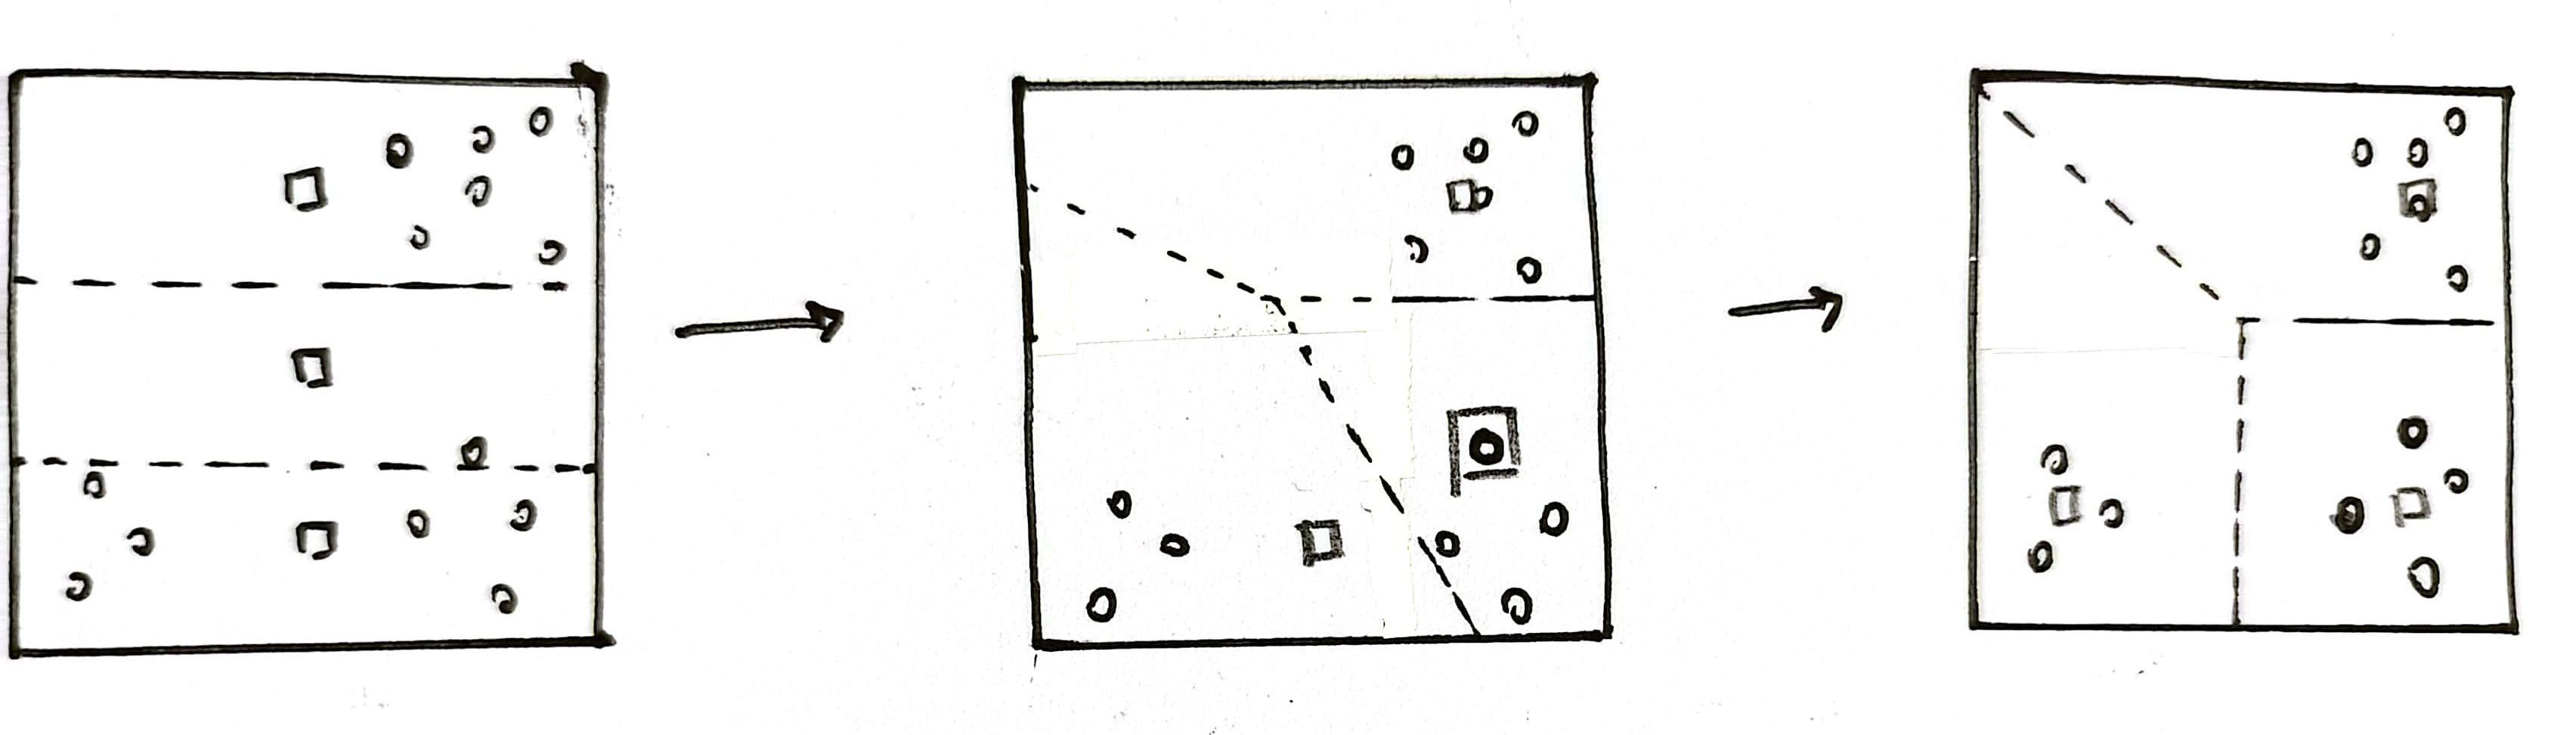
\includegraphics[scale=0.14]{习题5第六题.jpg}
    \end{figure}
\end{solution}
\begin{solution}[8.]
求解结果及Python代码如下:
\begin{table}[htbp]
    \centering
\begin{tabular}{cllllll}
        \toprule
\textbf{迭代次数} & \multicolumn{1}{c}{\textbf{A正面期望}} & \multicolumn{1}{c}{\textbf{A背面期望}} & \multicolumn{1}{c}{\textbf{B正面期望}} & \multicolumn{1}{c}{\textbf{B背面期望}} & \multicolumn{1}{c}{\textbf{A正面概率}} & \multicolumn{1}{c}{\textbf{B正面概率}} \\
        \midrule
\textbf{1}    & 6.82                               & 18.19                              & 17.18                              & 7.81                               & 0.27                               & 0.69                               \\
        \midrule
\textbf{2}    & 5.82                               & 17.2                               & 18.18                              & 8.8                                & 0.25                               & 0.67                               \\
        \midrule
\textbf{3}    & 4.99                               & 16.32                              & 19.01                              & 9.68                               & 0.23                               & 0.66                               \\
        \midrule
\textbf{4}    & 4.27                               & 15.53                              & 19.73                              & 10.47                              & 0.22                               & 0.65                               \\
        \midrule
\textbf{5}    & 3.59                               & 14.75                              & 20.41                              & 11.25                              & 0.2                                & 0.64                               \\
        \midrule
\textbf{6}    & 2.92                               & 13.95                              & 21.08                              & 12.05                              & 0.17                               & 0.64                               \\
        \midrule
\textbf{7}    & 2.21                               & 13.04                              & 21.79                              & 12.96                              & 0.14                               & 0.63                               \\
        \midrule
\textbf{8}    & 1.39                               & 11.96                              & 22.61                              & 14.04                              & 0.1                                & 0.62                               \\
        \midrule
\textbf{9}    & 0.52                               & 10.75                              & 23.48                              & 15.25                              & 0.05                               & 0.61                               \\
        \midrule
\textbf{10}   & 0.03                               & 10.04                              & 23.97                              & 15.96                              & 0                                  & 0.6                               \\
        \bottomrule
\end{tabular}
\end{table}
\begin{pythoncode}
import numpy as np
import pandas as pd

# 绘制表格参数
cols = ['A正面期望', 'A背面期望', 'B正面期望', 'B背面期望', 'A正面概率', 'B正面概率']
df = pd.DataFrame(columns=cols)  # 绘制表格

T = 10  # 总迭代次数
prA, prB = 0.3, 0.7  # 硬币A,B正面朝上的概率
samples = [4, 6, 0, 9, 5]  # 每个样本中正面朝上的个数
for _ in range(T):
    expectA, expectB = np.zeros(2), np.zeros(2)  # 硬币A,B的期望
    for i in range(len(samples)):
        tmp1 = np.power(prA, samples[i]) * np.power(1 - prA, 10 - samples[i])
        tmp2 = np.power(prB, samples[i]) * np.power(1 - prB, 10 - samples[i])
        chooseA = tmp1 / (tmp1 + tmp2)  # 选择硬币A的概率
        chooseB = 1 - chooseA  # 选择硬币B的概率
        expectA += np.array([samples[i] * chooseA, (10 - samples[i]) * chooseA])
        expectB += np.array([samples[i] * chooseB, (10 - samples[i]) * chooseB])
    prA = expectA[0] / np.sum(expectA)
    prB = expectB[0] / np.sum(expectB)
    tmp = pd.DataFrame(
        np.concatenate((expectA, expectB, np.array([prA]), np.array([prB]))).reshape([1, -1]),
        columns=cols)
    df = pd.concat([df, tmp])
df = df.reset_index(drop=True)
df.index += 1
df.index.name = '迭代次数'
print(df)
df.round(2).to_excel('ans8.xlsx')
\end{pythoncode}
\end{solution}
\begin{solution}[9.]
    K均值聚类算法可视为一种特殊的EM算法,聚类质心视为隐变量,求期望步骤中,通过计算欧氏距离判断每个样本点属于哪个聚类质心;在期望最大化中,通过计算均值,更新聚类质心位置,从而减小样本点到聚类质心的方差,增大属于该聚类质心的期望.
\end{solution}

% 正文部分

% 下面给一些功能的写法
\iffalse
% 图片模板
\centerline{
    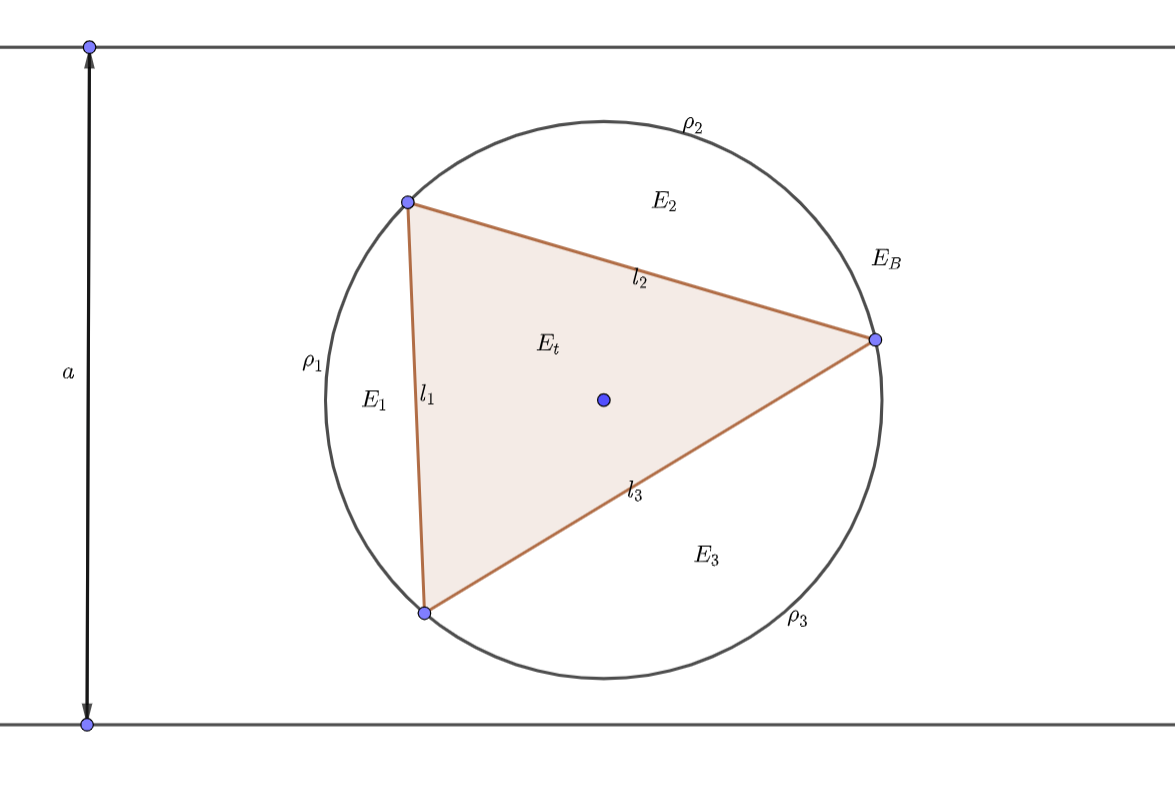
\includegraphics[width=0.8\textwidth]{figure.png}
}
% 表格模板
\renewcommand\arraystretch{0.8} % 设置表格高度为原来的0.8倍
\begin{table}[!htbp] % table标准
    \centering % 表格居中
    \begin{tabular}{p{1cm}<{\centering}p{1cm}<{\centering}p{3cm}<{\centering}p{5cm}<{\centering}} % 设置表格宽度
    %\begin{tabular}{cccc}
        \toprule
        $x_i$ & $f[x_1]$ & $f[x_i,x_{i+1}]$ & $f[x_i,x_{i+1},x_{i+2}]$ \\
        \midrule
        $x_0$ & $f(x_0)$ &                  &                          \\
        $x_0$ & $f(x_0)$ & $f'(x_0)$        &                          \\
        $x_0$ & $f(x_1)$ & $\frac{f(x_1)-f(x_0)}{x_1-x_0}$ & $\frac{f(x_1)-f(x_0)}{(x_1-x_0)^2}-\frac{f'(x_0)}{x_1-x_0}$\\
        \bottomrule
    \end{tabular}
\end{table}

\def\Log{\text{Log}} % 一个简单的宏定义
$\Log$ % 调用方法
\fi

\end{document}